\section{Thermal Expansion}
\label{sec:thermalExpansion}

\begin{frame}{Thermal Expansion Motivation}
  \begin{itemize}
    \item Metallic fuels.
    \item PRISM designed by GE-Hitachi Nuclear Energy (GEH) \cite{GEFR793}.
    \item EBR-II designed and built by Argonne National Laboratory (ANL)
      \cite{PlentifulEnergy}.
      \begin{itemize}
        \item Full-power demonstrations from April 1986.
        \item Unprotected Loss-Of-Flow (ULOF).
        \item Unprotected Loss-Of-Heat-Sink (ULOHS).
      \end{itemize}
  \end{itemize}
\end{frame}

\begin{frame}{Simplified Thermal Expansion Model}
  \begin{itemize}
    \item Calculate dimensions once at the beginning of simulation.
    \item Radial expansion modeled as steel. Expand at $\texpstruct$.
    \item Axial expansion modeled as fuel. Expand at $\texpfuel$.
    \item Sodium volume allowed to ``float''.
    \item Expand all linear dimensions.
    \item Decrease local densities accordingly to preserve material.
  \end{itemize}
\end{frame}

\begin{frame}{Material Properties}
  \begin{figure}
    \centering
    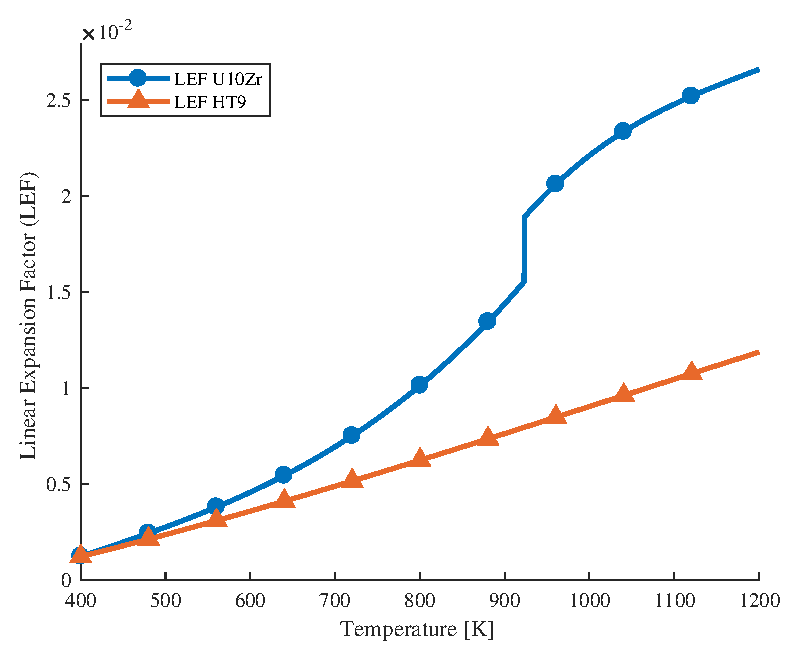
\includegraphics[width=0.7\textwidth]{lef_plot}
    \caption{Linear Expansion Factor for HT9 Steel and U10Zr Fuel.}
    \label{fig:lef_plot}
  \end{figure}
  %\begin{equation}
  %  \label{eq:lef_ht9}
  %  \left( \frac{\Delta L}{L} \right)_{\text{HT9}} = 
  %    -2.191 \times 10^{-3} + 5.678 \times 10^{-6} \, T + 
  %    8.111 \times 10^{-9} \, T^2 - 2.576 \times 10^{-12} \, T^3 ,
  %\end{equation}
  %\begin{multline}
  %  \label{eq:lef_u10zr}
  %  \left( \frac{\Delta L}{L} \right)_{\text{U10Zr}} = \\
  %    \begin{cases}
  %      -7.3 \times 10^{-3} + 3.489 \times 10^{-5} \, T 
  %        - 5.154 \times 10^{-8} \, T^2 + 4.39 \times 10^{-11} \, T^3 & 
  %        T \le 923 \units{K} \\
  %      -0.25252 + 6.669 \times 10^{-4} \, T - 5.441 \times 10^{-7} \, T^2 
  %        + 1.518 \times 10^{-10} \, T^3 & \text{otherwise}
  %    \end{cases}
  %\end{multline}
\end{frame}

\begin{frame}{Expansion Formulae}
  Given assumptions of uniform radial and axial expansion, volumes expand
  uniformly.
  \begin{equation}
    \label{eq:volume_ratio}
    \frac{V^C}{V^H} = \frac{1}{(1+F_r(\texpstruct))^2 (1+F_a(\texpfuel))}
  \end{equation}

  % TODO insert figure
\end{frame}

\begin{frame}{Expansion Formulae}
  \begin{itemize}
    \item Area fraction expansion ratios are more difficult.
    \item $a_j^C$ and $a_j^H$ are calculated explicitly.
    \item The volume occupied by material $j$ is the product of the 
      area fraction of the material and the volume of the element.
  \end{itemize}

  To preserve the number of atoms in the reactor, the number density must be
  diluted.
  \begin{equation}
    \label{eq:nden_thexp_update}
    N_i^H = N_i^C \frac{a_j^C}{a_j^H} 
      \frac{1}{(1+F_r(\texpstruct))^2 (1+F_a(\texpfuel))}
  \end{equation}

  Then cross-sections are proportional to number densities.
  \begin{equation}
    \Sigma = \sigma \, N
  \end{equation}
\end{frame}

\begin{frame}{Demonstration of Reactor Thermal Expansion}
  \begin{figure}
    \centering
    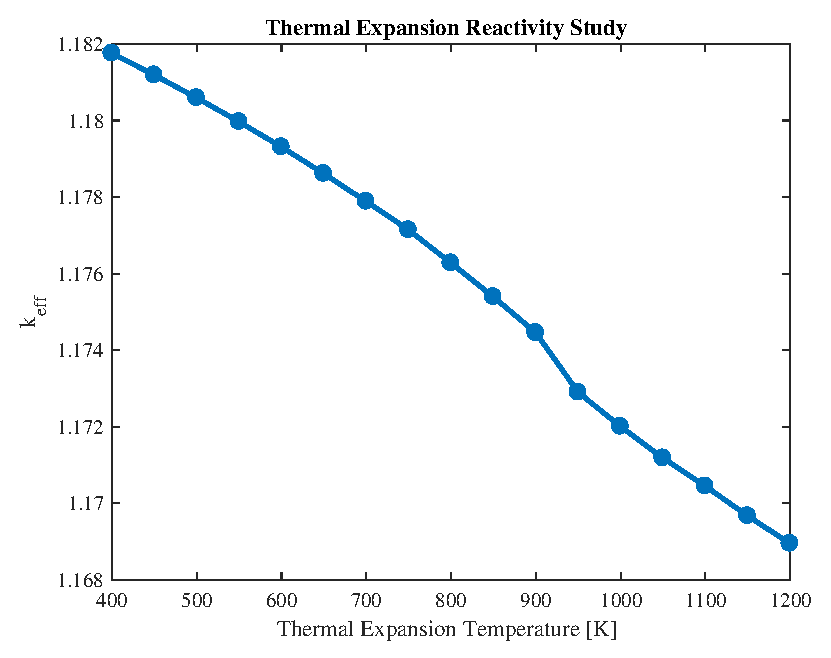
\includegraphics[width=0.7\textwidth]{thexp_study}
    \caption{Effective Neutron Multiplication Factor as a Function of 
      Thermal Expansion Temperature.}
    \label{fig:thexp_study}
  \end{figure}
  \begin{equation}
    \label{eq:reactivity_formula}
    \rho \units{pcm} = \frac{\keff - \kref}{\keff \, \kref} \times 10^5
  \end{equation}
\end{frame}
